% FEUP THESIS STYLE for LaTeX2e
% how to use feupteses (changed from the original for MIEEC)
%
% FEUP, JCL & JCF, Tue May 20 18:53:15 2008
%
% PLEASE send improvements to jlopes at fe.up.pt, jcf at fe.up.pt
%

%%========================================
%% Commands: pdflatex mieic
%%           bibtex mieic
%%           makeindex mieic (only if crating an index)
%%           pdflatex mieic
%%========================================

%% For one side layout comment next line and uncomment the second line
\documentclass[11pt,a4paper,twoside,openright]{report}
%\documentclass[11pt,a4paper]{report}

%% For iso-8859-1 (latin1), comment next line and uncomment the second line
\usepackage[utf8]{inputenc}
%\usepackage[latin1]{inputenc}

%% Use option portuges if needed
\usepackage[english]{babel}

%% For the final version, comment next line and uncomment the second line
\usepackage[provisional,alpharefs]{feupteses}
%\usepackage[alpharefs]{feupteses}

%% Options:
%% - portuges: titles, etc in portuguese
%% - provisional: the thesis has not been approved yet
%% - usewatermark: use watermark instaed of provisonal text
%% - print: links are not shown (for paper versions)
%% - alpharefs: bibliography references are alphabetic
%% - numericrefs: bibliography references are numbered (in order of citation)
%% ( by default: author-date format of the ``natbib'' package is used
%%   the portuguese version requires the file ``plainnat-pt.bst'' to be
%%   present in the same directory )

%% Include MIEIC definitions different from standard style
\usepackage{mieicpatch}

\usepackage{float}
\usepackage{subfig}
\usepackage[final=true,step=1]{microtype}
%\usepackage{lmodern}
\usepackage{longtable}
\usepackage{lscape}

\usepackage{color}
\definecolor{cloudwhite}{cmyk}{0,0,0,0.025}

\usepackage{listings}
\lstset{ %
 language=C,                        				    % choose the language of the code
 basicstyle=\footnotesize\ttfamily,
 keywordstyle=\bfseries,
 numbers=left,                   					      % where to put the line-numbers
 numberstyle=\scriptsize\texttt,    				    % the size of the fonts that are used for the line-numbers
 stepnumber=1,                      				    % the step between two line-numbers. If it's 1 each line will be numbered
 numbersep=8pt,                     				    % how far the line-numbers are from the code
 frame=tb,
 float=htb,
 aboveskip=8mm,
 belowskip=4mm,
 backgroundcolor=\color{cloudwhite},
 showspaces=false,                  				    % show spaces adding particular underscores
 showstringspaces=false,            				    % underline spaces within strings
 showtabs=false,                    				    % show tabs within strings adding particular underscores
 tabsize=2,	                        				    % sets default tabsize to 2 spaces
 captionpos=b,                      				    % sets the caption-position to bottom
 breaklines=true,                  				 	    % sets automatic line breaking
 breakatwhitespace=false,           				    % sets if automatic breaks should only happen at whitespace
 escapeinside={\%*}{*)},            				    % if you want to add a comment within your code
 morekeywords={*,Expect,var,template,new,...},  % if you want to add more keywords to the set
 literate={+}{{$+$}}1 {*}{{$*$}}1 {<=}{{$\leq$}}1 {>=}{{$\geq$}}1 {!=}{{$\neq$}}1 {==}{{$\equiv$}}1 {=>}{{$\leadsto$}}1
}

%% Provide a version number in order to keep track of
%% thesis versions (it will printed in the footer of most pages)

\version{0.99}

%% Uncomment in the final version in order to make version footer disappear
\noversiontrue

%% Uncomment to create an index (at the end of the document)
%\makeindex

%% Path to the figures directory
%% TIP: use folder ``figures'' to keep all your figures
\graphicspath{{figures/}}

%%----------------------------------------
%% TIP: if you want to define more macros, use an external file to
%% keep them
\include{mymacros}
%%----------------------------------------

%%========================================
%% Start of document
%%========================================
\begin{document}

%%----------------------------------------
%% Information about the work
%%----------------------------------------
\title{Improving Variability of Applications using Adaptive Object-Models}
\author{João Gradim Pereira}
\degree{Master in Informatics and Computing Engineering}
%% Date of submission
\thesisdate{17$^{th}$ January, 2011}

%% Insert copyright text if used
%\copyrightnotice{Name of the Author, 2008}

\supervisor{Supervisor}{Ademar Aguiar}{(Ph.D)}
%% Uncomment next line if necessary
\supervisor{Supervisor}{Hugo Sereno Ferreira}{(Ph.D AbD)}

%% Uncomment committee stuff in the final version
%\committeetext{Approved in oral examination by the committee:}
%\committeemember{Chair}{Name of the President}{(Title)}
%\committeemember{External Examiner}{Name of the Examiner}{(Title)}
%\committeemember{Supervisor}{Ademar Aguiar}{(Ph.D)}
%\signature
%\committeedate{31$^{st}$ July, 2010}

%% Specify cover logo (in folder ``figures'')
\logo{feup-logo.pdf}

%%----------------------------------------
%% Cover page(s)
%%----------------------------------------
\maketitle

%% Uncomment next line in the final version
\committeepage
%MIEEC uses an external PDF page with the signatures (juri.pdf)
%\includepdf[pagecommand={},noautoscale=false,fitpaper=true,pages=-]{juri.pdf}

%% Preliminary materials
\StartPrelim
\begin{singlespace}
  \chapter*{Abstract}

One particular point of interest is to allow the end-users to modify the system definition --- which implies these modifications have to be performed without any programming or system redeploying.

An Adaptive Object-Model architecture is a system architecture that represents classes, attributes, relationships, and behavior as \emph{metadata}.

\chapter*{Resumo}


 % the abstract
  %\chapter*{Acknowledgements}

\vspace{10mm}
\flushleft{O Autor}

  % the acknowledgments
  \cleardoublepage
\thispagestyle{plain}

\vspace*{8cm}

\begin{flushright}
   \textsl{``Computers are good at reading instructions, not at reading your mind''} \\
\vspace*{1.5cm}
           Donald E. Knuth
\end{flushright}

    % initial quotation if desired
  \cleardoublepage
  \pdfbookmark[0]{Table of Contents}{contents}
  \tableofcontents
  \cleardoublepage
  \pdfbookmark[0]{List of Figures}{figures}
  \listoffigures
  \cleardoublepage
  \pdfbookmark[0]{List of Tables}{tables}
  \listoftables
  \cleardoublepage
  \pdfbookmark[0]{Abbreviations}{abbrevs}
  \chapter*{Abbreviations}
%\addcontentsline{toc}{chapter}{Abbreviations}
\chaptermark{Abbreviations}

\begin{flushleft}
\begin{tabular}{l p{0.8\linewidth}}
AOP       & Aspect-Oriented Programming\\
API       & Application Programming Interface\\
CRUD      & Create, Read, Update, Delete\\
DSL       & Domain Specific Language\\
DSML      & Domain Specific Modeling Language\\
GUI       & Graphical User Interface\\
MVC       & Model, View, Controller (design pattern)\\
OOP       & Object-Oriented Programming\\
PIM       & Platform-Independent Model\\
RoR       & Ruby on Rails\\
UI        & User Interface\\
UML       & Unified Modeling Language\\
\end{tabular}
\end{flushleft}

  % the list of abbreviations used
\end{singlespace}

%%----------------------------------------
%% Body
%%----------------------------------------
\StartBody

%% TIP: use a separate file for each chapter
\chapter{Introduction}\label{chap:intro}

\section{Context}\label{sec:context}

Software systems are usually designed with a specific purpose in mind. They rely on a series of requirements which are often very difficult to capture and maintain, as they have a tendency to evolve faster than the implementation. This is caused mainly by the poor understanding by the stakeholders about their needs and expectations about what a software system should be able to do~\cite{PT07}. These situations lead to higher costs in software development, as creating and maintaining software systems is a knowledge intensive task~\cite{AdOdSBD07}. Moreover, most of these system are not static, and have a constant need to evolve in order to adapt themselves to their environment and new business rules, shifting the stakeholders' needs and expectations about these software systems.

In face of these situations, new development methods started to focus more on iterative and incremental approaches, accepting \textit{incompleteness} as part of every software system development cycle~\cite{WC03}. At the same time, many new systems are being developed with an emphasizis on flexibility and run-time configuration~\cite{YJ02}. These approaches present a clear contrast with an up-front, full specification for a software system, which, albeit benefitial for some cases, are impratical in constant evolution scenarios. This leads to a change in software requirements and inevitable refactoring, which in turn may lead to a \textsc{big ball of mud}, ultimately leading to unmaintainable systems, very costly to modify and adapt to the stakeholders needs~\cite{FY97}.

\section{Motivation and Objectives}\label{sec:goals}

Developing quality software is a costly process. Maintaining, as well as adding new features to these software systems is a costly and time-consuming process. If the end-user is allowed to make changes to an information system in runtime, it can effectively shape the system's architecture (model and relation-wise) to suit his or her needs according to the natural evolution of the business rules, enviroment changes and needs.

This project will be applied to the \textit{Escolinhas}~\cite{escolinhas}, a growing, Portuguese, Ruby On Rails based project. Escolinhas aims at sustaining social and collaborative work for children in elementary schools involving students, teachers and parents as its users. With the teachers demanding better and more adaptable teaching tools, it becomes an excellent case-study application to research, test and apply all the work and discoveries made during the course of this thesis.

% Establish a reference framework using the concepts of web 2.0 for AOM systems
% Understand GUI patterns that allow end-users to manipulate domain models
% Validate through an industrial use-case application

\section{Report Overview}\label{sec:structure}

The rest of this report is structured as follows:\\

%\textbf{Chapter \ref{chap:technologies}: ``\nameref{chap:technologies}'' } presents the main technologies which will be part of the development process.\\

\textbf{Chapter \ref{chap:sota}: ``\nameref{chap:sota}'' } reviews the most important methodologies and patterns used to make software as adaptable and maintable as possible.\\

\textbf{Chapter \ref{chap:problem_statement}: ``\nameref{chap:problem_statement}'' } exposes the problem to be addressed and thoroughly explains it, while explaining it usefulness.\\

\textbf{Chapter \ref{chap:approach_results}: ``\nameref{chap:approach_results}'' } reviews the current design of the platform, and performs a variability analysis of the system, choosing three focus areas. Then, for each one of the areas, demonstrates its variability requirements, candidate patterns, the chosen patterns and rationale behind such decisions, implementation details and impact analysis.\\

\textbf{Chapter \ref{chap:validation}: ``\nameref{chap:validation}'' } validates the work described in Chapter~\ref{chap:approach_results} through various metrics\\ % FIXME

\textbf{Chapter \ref{chap:conclusions}: ``\nameref{chap:conclusions}'' } reviews the project, drawing conclusions about the issues addressed in Chapters \ref{chap:approach_results} and \ref{chap:validation}. It also provides a summary of contributions and some insights on which future developments have been considered.
\\











%\chapter{Technologies}\label{chap:technologies}

\section{C\#}\label{sec:csharp}

\section{Oghma}\label{sec:oghma}

\section{Ruby}\label{sec:technologies:ruby}

\section{HTML}\label{sec:html}

\section{Javascript}\label{sec:javascript}


%% FEUP THESIS STYLE for LaTeX2e
%% how to use feupteses (changed from the original for MIEEC)
%%
%% FEUP, JCL & JCF, Sun Jan 18 21:34:13 2009
%% Version v2009-rc1 (MIEEC)
%%
%% PLEASE send improvements to jlopes at fe.up.pt, jcf at fe.up.pt
%%

%%========================================
%% Commands: pdflatex tese
%%           bibtex tese
%%           makeindex tese (only if creating an index) 
%%           pdflatex tese
%%========================================

\documentclass[11pt,a4paper,twoside,openright]{report}

%% For iso-8858-1 (latin1), comment next line and uncomment the second line
\usepackage[utf8]{inputenc}
%\usepackage[latin1]{inputenc}

%% Use option portuges if needed
\usepackage[english]{babel}

%% For the final version, comment next line and uncomment the second line
\usepackage[portuges,provisional,numericrefs]{feupteses}
%\usepackage[portuges]{feupteses} 

%% Options: 
%% - portuges: titles, etc in portuguese
%% - provisional: the thesis has not been approved yet
%% - alpharefs: bibliography references are alphabetic (style
%%   alpha-pt.bst must be present in the same directory as the
%%   document sources)
%% - numericrefs: bibliography references are numbered (in order of citation)
%% ( by default: author-date format of the ``natbib'' package is used.
%%   The portuguese version requires the file ``plainnat-pt.bst'' to be 
%%   present in the same directory as the document sources.)

%% Provide a version number in order to keep track of
%% thesis versions (it will printed in the footer of most pages)

\version{0.99}

%% The version will automatically ``disappear'' in the final
%% (non-provisional) version of the document.

%% Uncomment to create an index (at the end of the document)
%\makeindex

%% path to the figures directory
%% TIP: use folder ``figures'' to keep all your figures
\graphicspath{{figures/}}

%%----------------------------------------
%% TIP: if you want to define more macros, use an external file to
%% keep them
\include{mymacros}
%%----------------------------------------

%%========================================
%% Start of document
%%========================================
\begin{document}

%%----------------------------------------
%% Information about the work
%%----------------------------------------
\title{End-User Reconfiguration of Applications using Adaptive Object-Models}
\author{João Gradim Pereira}
\degree{Mestrado Integrado em Engenharia Informática}
%% Date of submission
\thesisdate{July 16 2010}

%% insert copyright text if used
\copyrightnotice{João Gradim Pereira, 2010}

\supervisor{Supervisor}{Ademar Aguiar}{(Ph.D)}
%% Uncomment next line if necessary
\supervisor{Co-supervisor}{Hugo Sereno Ferreira}{(Ph.D. AbD)}

%% Uncomment committee stuff in the final version if used
%\committeetext{Aprovado em provas públicas pelo Júri:}
%\committeemember{Presidente}{Nome do presidente do júri}{(Título)}
%\signature
%\committeemember{Arguente}{Nome do arguente do júri}{(Título)}
%\signature
%\committeemember{Vogal}{Nome do vogal do júri}{(Título)}
%\signature
%\committeedate{31 de Julho de 2009}

%% specify cover logo (in folder ``figures'')
\logo{feup-logo.png}

%%----------------------------------------
%% Cover page(s)
%%----------------------------------------
\maketitle
%% Uncomment next line in the final version if used
%\committeepage

%% Preliminary materials
\StartPrelim
\begin{singlespace}
  \chapter*{Abstract}

One particular point of interest is to allow the end-users to modify the system definition --- which implies these modifications have to be performed without any programming or system redeploying.

An Adaptive Object-Model architecture is a system architecture that represents classes, attributes, relationships, and behavior as \emph{metadata}.

\chapter*{Resumo}


 % the abstract
  \chapter*{Acknowledgements}

\vspace{10mm}
\flushleft{O Autor}

  % the acknowledgments
  \cleardoublepage
\thispagestyle{plain}

\vspace*{8cm}

\begin{flushright}
   \textsl{``Computers are good at reading instructions, not at reading your mind''} \\
\vspace*{1.5cm}
           Donald E. Knuth
\end{flushright}

    % initial quotation if desired
  \cleardoublepage
  \pdfbookmark[0]{Contents}{contents}
  \tableofcontents
  \cleardoublepage
   \pdfbookmark[0]{List of Figures}{figures}
  \listoffigures
  \cleardoublepage
  \pdfbookmark[0]{List of Tables}{tables}
  \listoftables
  \chapter*{Abbreviations}
%\addcontentsline{toc}{chapter}{Abbreviations}
\chaptermark{Abbreviations}

\begin{flushleft}
\begin{tabular}{l p{0.8\linewidth}}
AOP       & Aspect-Oriented Programming\\
API       & Application Programming Interface\\
CRUD      & Create, Read, Update, Delete\\
DSL       & Domain Specific Language\\
DSML      & Domain Specific Modeling Language\\
GUI       & Graphical User Interface\\
MVC       & Model, View, Controller (design pattern)\\
OOP       & Object-Oriented Programming\\
PIM       & Platform-Independent Model\\
RoR       & Ruby on Rails\\
UI        & User Interface\\
UML       & Unified Modeling Language\\
\end{tabular}
\end{flushleft}

  % the list of abbreviations used
\end{singlespace}

%%----------------------------------------
%% Body
%%----------------------------------------
\StartBody

%% TIP: use a separate  file for each
\chapter{Introduction}\label{chap:intro}

\section{Context}\label{sec:context}

\begin{quote}
  ``Like the Abstract, the Introduction should be written to engage the
  interest of the reader. It should also give the reader an idea of
  how the dissertation is structured, and in doing so, define the
  thread of the contents.''~\citep[chap.\ Introduction]{kn:Tha01}
\end{quote}

\section{Motivation and Objectives}\label{sec:goals}

\section{Report Overview}\label{sec:structure}

 
\chapter{State Of The Art in Adaptive Systems}

\section{Generative Programming}

\subsection{Model-Driven Architectures}

\subsection{Ruby On Rails}

\subsection{Frameworks}

%-------------------------------------------------------------------------------

\section{Meta-Architecture}

\subsection{Meta Programming}

\subsection{Smalltalk}

\subsection{Ruby}

\subsection{Adaptive Object-Models}


\chapter{Approach}\label{chap:approach}

As stated in Section \ref{sec:goals}, the main objective of this thesis is to bring the Oghma framework to a web environment. This section describes the work plan for the project that will serve as the basis for the dissertation writing.

\section{Work Plan}\label{sec:work_plan}

\begin{figure}[H]
  \includegraphics[width=165mm]{work_plan_small.png}
  \caption{Work plan for the duration of the thesis}
  \label{fig:work_plan}
\end{figure}


\chapter{Mais um Capítulo}\label{chap:chap4}

\section*{}

Neste capítulo mostra-se apenas o formato da dissertação.

Ipsum dolor sit amet, consectetuer
adipiscing elit.  Praesent sit amet sem. 
Maecenas eleifend facilisis leo. Vestibulum et
mi. Aliquam posuere, ante non tristique consectetuer, dui elit
scelerisque augue, eu vehicula nibh nisi ac est. 
Suspendisse elementum sodales felis. 
Nullam laoreet fermentum urna. 

\section{Secção Exemplo}

Lorem ipsum dolor sit amet, consectetuer adipiscing elit. Integer
hendrerit commodo ante. Pellentesque nibh libero, aliquam at, faucibus
id, commodo a, velit. Duis eleifend sem eget leo. Morbi in
est. Suspendisse magna sem, varius nec, hendrerit non, tincidunt quis,
quam. Aenean congue. Vivamus vel est sit amet sem iaculis
posuere. Cras mollis, enim vel gravida aliquam, libero nunc
ullamcorper dui, ullamcorper sodales lectus nulla sed urna. Morbi
aliquet porta risus. Proin vestibulum ligula a purus. Maecenas a
nulla. Maecenas mattis est vitae neque auctor tempus. Etiam nulla dui,
mattis vitae, porttitor sed, aliquet ut, enim. Cras nisl magna,
aliquet et, laoreet at, gravida ac, neque. Sed id est. Nulla dapibus
dolor quis ipsum rhoncus cursus. 

Etiam nisi est, dignissim sodales, fermentum id, pulvinar ac,
eros. Duis id orci. Nam pretium nisl ac augue. Ut adipiscing magna
eget est. Curabitur varius. Nulla facilisi. Pellentesque sit amet
neque ac dui accumsan blandit. Donec mauris felis, egestas sit amet,
convallis ac, dignissim quis, dolor. Maecenas cursus tortor vel
leo. Quisque tristique. Nunc augue odio, tincidunt in, dapibus sed,
ultricies sit amet, lorem. In hac habitasse platea dictumst. Praesent
iaculis, lacus hendrerit tempor sodales, libero tellus aliquet orci,
ut rhoncus massa lectus quis erat. Pellentesque quis dolor nec tortor
rhoncus convallis. Aliquam erat volutpat. Fusce placerat, magna eu
imperdiet lobortis, augue massa blandit turpis, a consectetuer quam
arcu sit amet risus. Suspendisse potenti. Praesent sapien metus,
interdum vitae, fermentum id, faucibus ut, lorem. Nunc iaculis purus
id tortor. Aenean risus pede, laoreet ac, tristique sed, lobortis in,
turpis. 

Vestibulum et lorem in ligula viverra pharetra. Curabitur quis purus
in urna facilisis bibendum. Pellentesque at arcu accumsan velit
bibendum ornare. Praesent massa. Quisque dolor. In libero. Vestibulum
ac diam id leo feugiat blandit. Donec porta, tellus ac pellentesque
molestie, felis mauris viverra lacus, sed dignissim purus justo eu
justo. Proin iaculis, nunc eu volutpat volutpat, libero purus rutrum
enim, id euismod lacus lorem nec augue. Donec hendrerit lacinia
ante. Integer mollis vulputate orci. In pellentesque, metus pharetra
elementum pharetra, est purus bibendum turpis, eu pretium sapien
libero convallis odio. Cras sodales bibendum risus. Sed mattis nulla
non leo. Nulla nunc. Phasellus egestas sodales massa. Class aptent
taciti sociosqu ad litora torquent per conubia nostra, per inceptos
himenaeos. Pellentesque habitant morbi tristique senectus et netus et
malesuada fames ac turpis egestas. Etiam mi. 

\section{Mais uma Secção}

Lorem ipsum dolor sit amet, consectetuer adipiscing elit. Quisque
purus sapien, interdum ut, vestibulum a, accumsan ullamcorper,
erat. Mauris a magna ut leo porta imperdiet. Donec dui odio, porta in,
pretium non, semper quis, orci. Quisque erat diam, pharetra vel,
laoreet ac, hendrerit vel, enim. Donec tristique luctus risus. Fusce
dolor est, eleifend id, elementum sit amet, varius vitae, neque. Morbi
at augue. Ut sem ligula, auctor vitae, facilisis id, pharetra non,
lectus. Nulla lacus augue, aliquam eget, sollicitudin sed, hendrerit
eu, leo. Suspendisse ac tortor. Mauris at odio. Etiam vehicula. Nam
lacinia purus at nibh. Aliquam fringilla lorem ac justo. Ut nec
enim. Nunc ornare, eros eu facilisis tristique, nisl lorem lacinia
risus, non ullamcorper tellus urna et eros. Quisque eleifend tempus
metus. Nunc ipsum. 

Phasellus ullamcorper justo id risus. Nunc in leo. Mauris auctor
lectus vitae est lacinia egestas. Nulla faucibus erat sit amet lectus
varius semper. Praesent ultrices vehicula orci. Nam at metus. Aenean
eget lorem nec purus feugiat molestie. Phasellus fringilla nulla ac
risus. Aliquam elementum aliquam velit. Aenean nunc odio, lobortis id,
dictum et, rutrum ac, ipsum. Aenean tellus magna, lacinia eget,
bibendum ut, interdum sit amet, ipsum. Class aptent taciti sociosqu ad
litora torquent per conubia nostra, per inceptos himenaeos. Mauris
felis lacus, dapibus sit amet, pretium feugiat, aliquet non,
purus. Aliquam elementum, diam quis porttitor gravida, sem sapien
iaculis nulla, ut pharetra odio felis a metus. Nulla lacus ipsum,
tristique ut, dapibus sed, mollis et, justo. Vivamus non ipsum sed
ligula placerat ultrices. Maecenas dictum leo adipiscing
mauris. Vestibulum tristique, lacus a consequat suscipit, nunc dui
sollicitudin arcu, non interdum libero est eget tortor. Ut eget neque
quis leo tempor dictum. 

Quisque ullamcorper. Aliquam vel magna. Sed pulvinar dictum
ligula. Sed ultrices dolor ut turpis. Vivamus sagittis orci malesuada
arcu venenatis auctor. Proin vehicula pharetra urna. Aliquam egestas
nunc quis nisl. Donec ullamcorper. Nulla purus. Ut suscipit lacus
vitae dui. Mauris semper. Ut eget sem. Integer orci. Nam vitae dui
eget nisi placerat convallis. 

Sed id lorem. Proin gravida bibendum lacus. Sed molestie, urna quis
euismod laoreet, diam dolor dictum diam, vitae consectetuer leo ipsum
id ante. Integer eu lectus non mauris pharetra viverra. In feugiat
libero ut massa. Morbi cursus, lorem sollicitudin blandit semper,
felis magna pellentesque lacus, ut rhoncus leo neque at tellus. Sed
mattis, diam eget eleifend tincidunt, ligula eros tincidunt diam,
vitae auctor turpis est vel nunc. In eu magna. Donec dolor metus,
egestas sit amet, ultrices in, faucibus sed, lectus. Etiam est enim,
vehicula pharetra, porta non, viverra vel, nunc. Ut non sem. Etiam nec
neque. Sed rhoncus, justo id imperdiet pharetra, mi tellus accumsan
neque, vitae volutpat tortor enim in odio. Nunc porta justo a
lorem. Nulla hendrerit odio vitae dolor. Suspendisse eu nisl.  

\section{Resumo ou Conclusões}

Proin vehicula pharetra urna. Aliquam egestas
nunc quis nisl. Donec ullamcorper. Nulla purus. Ut suscipit lacus
vitae dui. Mauris semper. Ut eget sem. Integer orci. Nam vitae dui
eget nisi placerat convallis. 

\chapter{Conclusions}\label{chap:concl}

 

%% Comment next 2 commands if numbered appendixes are not used
\appendix
\include{appendix1}

%%----------------------------------------
%% Final materials
%%----------------------------------------

\begin{singlespace}
  %% Bibliography
  %% Comment the next command if BibTeX file not used, 
  %% bibliography is in ``myrefs.bib''
  \PrintBib{myrefs}

  %% Index
  %% Uncomment next command if index is required, 
  %% don't forget to run ``makeindex tese'' command
  %\PrintIndex
\end{singlespace}

\end{document}

\chapter{Problem Statement}\label{chap:problem_statement}

While Ruby on Rails is built to maximize the developers productivity, it does so by providing a comprehensive set of tools that perform most of the work. The RoR framework is also designed for easy system evolution through \emph{migrations} --- which allow developers to easily add, remove and modify tables and table rows, while minimizing the effort of maintaining application consistency. While this is a solid, proven approach to improve an application's variability over time, it is often less flexible than one might wish, often leading to complicated data migration tasks which may involve modifying production data while ensuring consistency --- this can pose as a problem when the ammount of data is extensive and highly variable in nature. As such, the use of a static database schema coupled with migrations may not be entirely desireable for applications highly variable in nature.

As presented on Chapter~\ref{chap:sota}, the usage and application of adequate design patterns is capable of mitigating some of these issues, improving both an application's variability and maintainability.

The main concern of this thesis is how these architectural and design patterns can be effectively applied to a somewhat (architecturaly speaking) restrictive framework, and how these techniques can be combined with a schema-oriented MVC architecture used by the Ruby on Rails Framework.

FIXME: It is also concerned with how can the variability of such systems increase and how effective they are in terms of development and performance.

\section{Architectural Patterns}\label{sec:architectural_patterns}

The application of architectural patterns is outside the scope of this project, mainly because the project which will serve as a base to the case studies herein described is tied to the Ruby on Rails framework and its implementation of the MVC architecture for software systems. Trying to tackle the problem by changing the underlying architecture would mean that the application would mostly have to be rebuilt from scratch, with the team having to stop development to rewrite the application and learning a whole new set of skills, which is simply not feasible. FIXME: Also, financial issues with having the whole team (it's a small team) training instead of developing and enhancing the existing product. % Many companies are tied to obsolete software for the same reasons

\section{Design Patterns}\label{sec:design_patterns}

As the modification of the underlying architecture has been discarded for the reasons stated in \ref{sec:architectural_patterns}, the next step is to modify only \emph{parts} of the application design, focusing on a number of different areas --- or hotspots --- chosen for their unique requirements in terms of variability.

Which AOM-related design patterns should be applied to solve certain problems, and why


\chapter{Approach \& Results}\label{chap:approach_results}

\section{Current Design Analysis}\label{sec:current_design_analysis}

A thorough analysis of the current design of the application was the first step taken, in order to identify potential problems within the platform. This study was conducted using a series of tools\footnote{Rubymine 2.0\cite{rubymine}, Rails ERD\cite{rails_erd}} that, unfortunately (at the time of writing), proved unsuccessful in extracting an \emph{Entity Relationship Diagram} from the code of the application. As such, another approach was taken: the product owner of the platform was queried on what he felt were the variability ``hotspots'' of the application: this narrowed the scope of the current design analysis, allowing focus on three different areas, as stated in~\ref{sec:case-study_areas}. These areas were then manually studied in order to extract the \emph{Entity Relationship Diagrams} relative to each one, which allowed analyzing each one as independently as possible, so that the applied design patterns (if any) would emerge --- making the task of pinpointing exactly what was wrong with each approach much easier.

\section{Variability Analysis}\label{sec:variability_analysis}

Each one of the areas (Roles, Social Network and the Document Editor) referred in \ref{sec:case-study_areas} was then studied in order to determine their variability requirements, and to which degree this variability should exist: developer, system administrator, or even end-user. These requirements were defined by the carefully considering the opinions from the users of the platform, the product owner and the main developers. These requirements were then used to determine which design patterns would be more appropriate to achieve the problems posed by each of the areas, and why.

\section{Implementation \& Impact Analysis}

For each one the three focus areas, functional prototypes were developed, either directly on top of the platform (Social Network, \ref{sec:fa_social_network}, and User Roles, \ref{sec:fa_roles}) or as an independent proof-of-concept application (Document Editor, \ref{sec:fa_documents}), that, as soon as possible, will be integrated into the main platform. These prototypes, however simplistic (and not yet in production), will be able to validate the research and decisions made throughout the next sections. All of the prototypes are implemented using Ruby 1.9.1 and Rails 2.3.9, as used in the production and development environments of \emph{escolinhas.pt}.

The impact analysis for each of these areas will be made in two different fronts: variability and performance. Variability impact analysis will be concerned with the increase in flexibility/configurability of a certain component, and how it measures to the objectives established beforehand. Performance analysis will (if applicable) examine the how much more (or less) performant each one of the implementations is, compared to the previous solutions.

\section{User Roles}\label{sec:fa_roles}

\subsection{Variability Requirements}\label{sec:fa_roles_variability_requirements}

\subsection{Candidate Patterns}\label{sec:fa_roles_candidate_patterns}

\subsection{Chosen Patterns \& Rationale}\label{sec:fa_roles_chosen_patterns_rationale}

\subsection{Implementation}\label{sec:fa_roles_implementation}

\subsection{Impact Analysis}\label{sec:fa_roles_impact_analysis}

\section{Social Network}\label{sec:fa_social_network}

As a social platform, \emph{escolinhas.pt} makes heavy use of the social network created by its users. Due to the nature of the application, which closely mimics the Portuguese primary school system, there is a need to control how the users (especially the students and parents) interact with each other; in other words, the application needs to have mechanisms that allow the manipulation of the social network. This section describes the study and work involved in creating such mechanisms, as well as implementation details and its impact details, both in terms of variability and performance.

\subsection{Variability Requirements}\label{sec:fa_social_network_variability_requirements}

The current design for the escolinhas.pt social network is based on the relationships formed through the connections between users and their schools, groups, and other users, as depicted in Fig.~\ref{fig:social_network_current}. The User's Roles play an important part in the definition of this network, as an user is only linked directly to other users; any other connection is mediated through their Roles, creating their association with Schools and Groups. This allows the construction of a network where all the connections can be inferred dynamically and where an user can be identified to another through these same connections: friends, classmates, parent--child, teacher--student, and so on. This network is used mainly in the internal communication systems of \emph{escolinhas.pt}, which allows users to communicate with each other within the platform.

\begin{figure}[H]
  \centering
  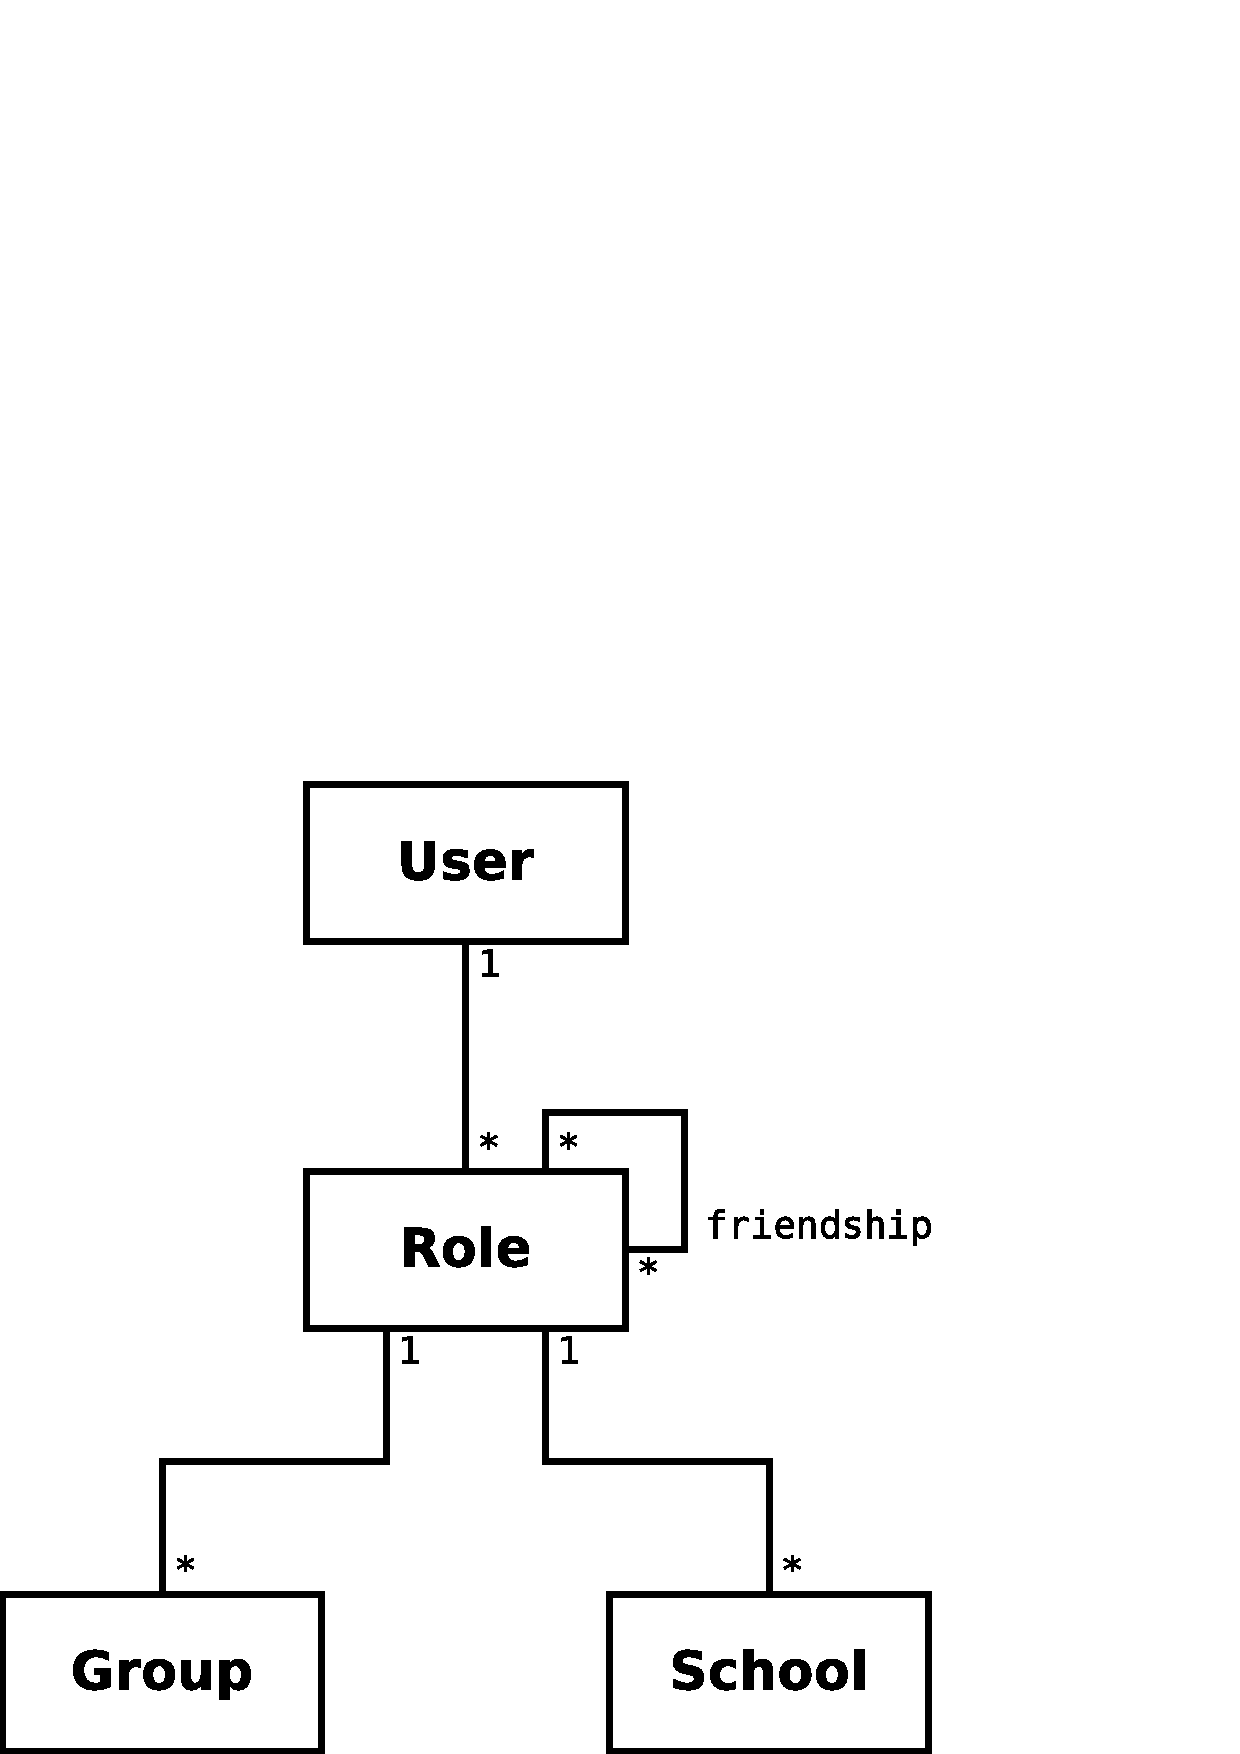
\includegraphics[width=65mm]{social_network_current.pdf}
  \caption{Current User Network Model.}
  \label{fig:social_network_current}
\end{figure}

This model, however useful, offers a very small degree of variability. Due to the closed nature of the platform, there is a need to provide mechanisms able to fine-tune these connections in order to accommodate to each school specific needs --- some Schools may not want to appear in search results; there may be some Students or even Parents who need to have special communication privileges. These mechanisms need to be available at the system administrator level, in order to easily manipulate these links without the need to pollute the application's codebase with hard-coded rules and without the need for redeployement.

\subsection{Candidate Patterns}\label{sec:fa_social_network_candidate_patterns}

Ideally, the user network would be described with a simple, self-referencing model, as shown in figure~\ref{fig:ideal_social_network_users}. This would allow the creation of static relationships between any two users that could be edited as needed. This would work great if all that was needed was to create relationships between users. However, it is often necessary to create connections between users and other entities in the system, such as groups and schools. Thus, this simple model needs to be abstracted in order to connect any two entities present in the system, whichever they may be, as shown in Fig.~\ref{fig:ideal_social_network_things}.

\begin{figure}[H]
  \centering
  \subfloat[Users Network]{\label{fig:ideal_social_network_users}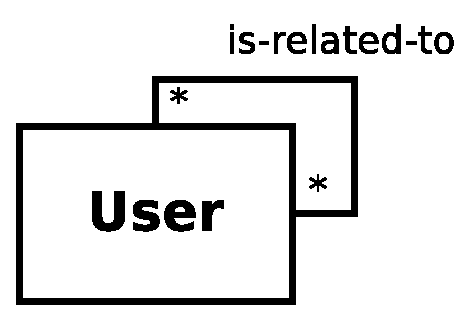
\includegraphics[width=35mm]{ideal_social_network_users}}
  \hspace{20mm}
  \subfloat[Entities Network]{\label{fig:ideal_social_network_things}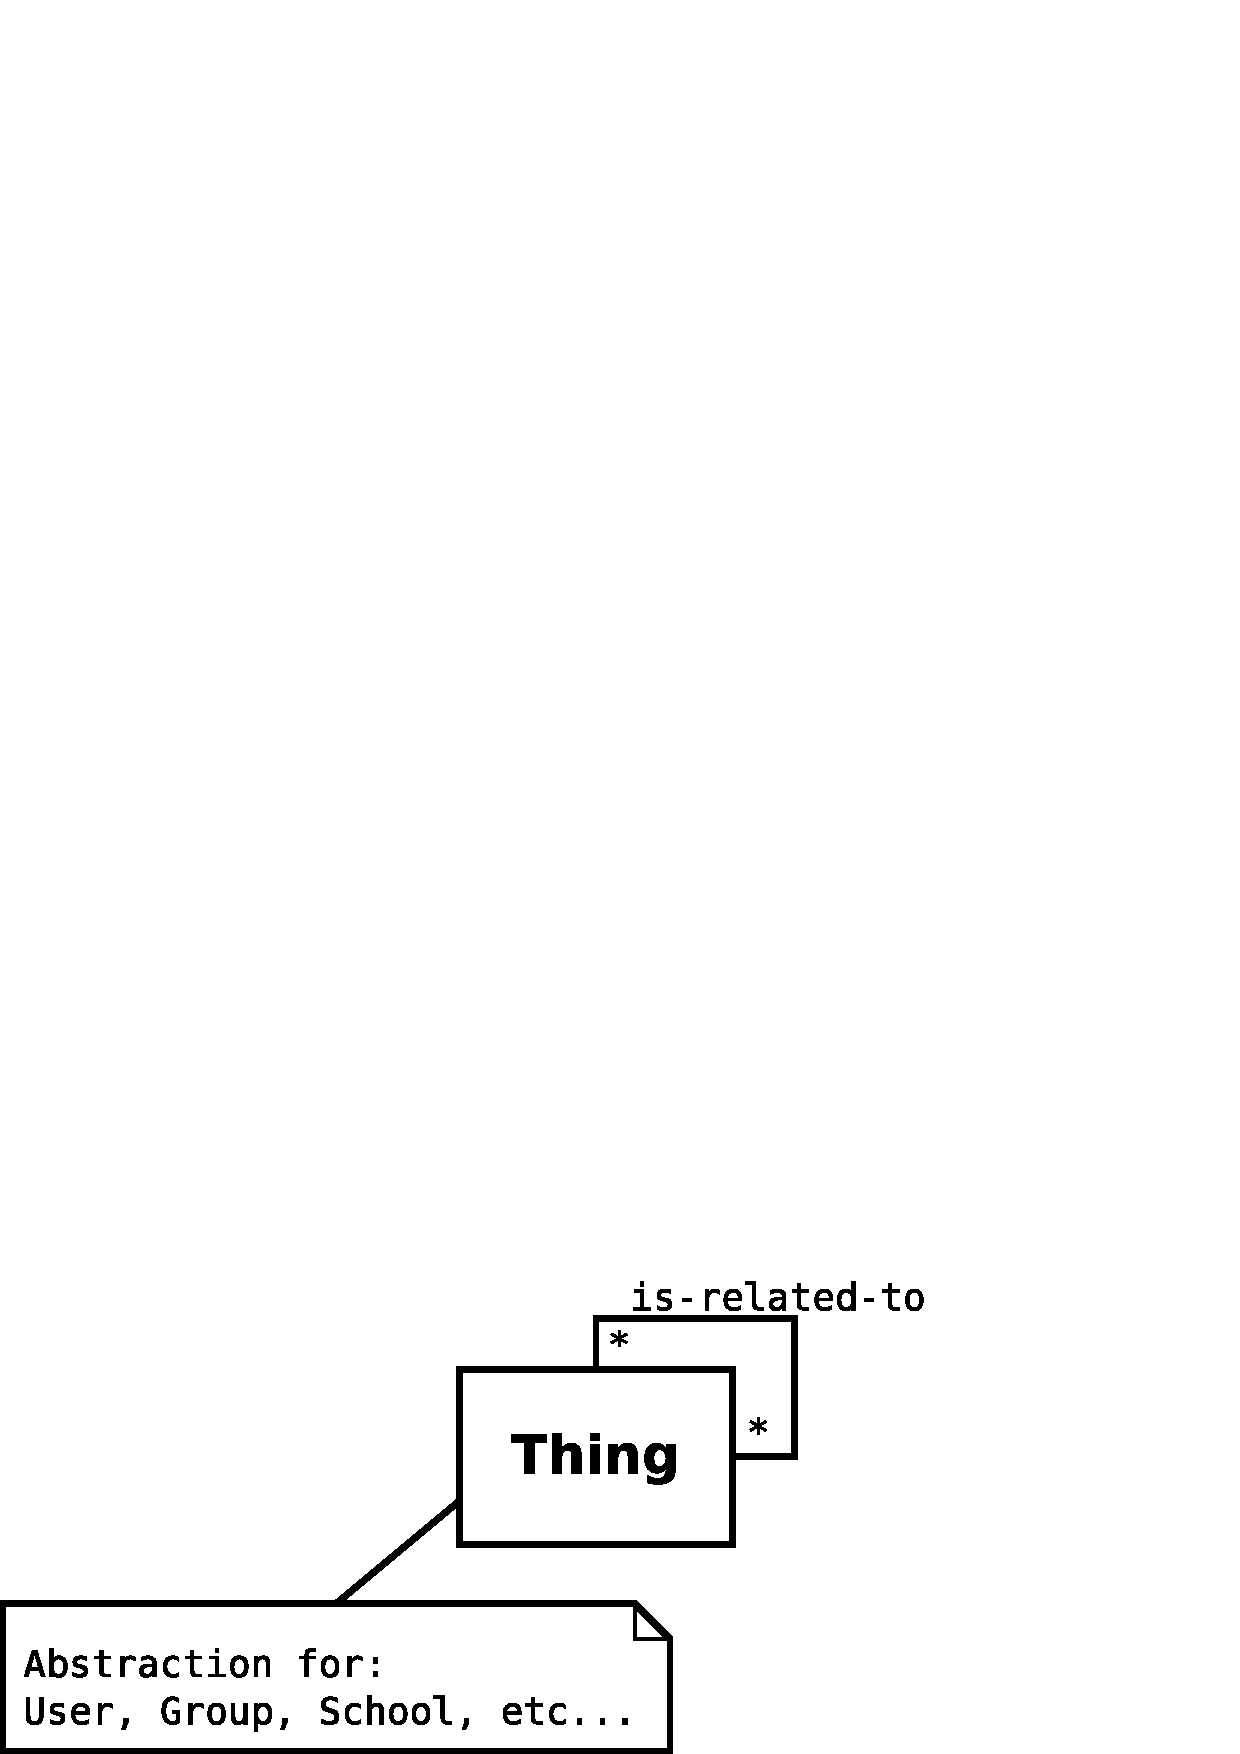
\includegraphics[width=65mm]{ideal_social_network_things}}
  \caption{Simplified Network Models.}
  \label{fig:simplified_network_models}
\end{figure}

\subsection{Chosen Patterns \& Rationale}\label{sec:fa_social_network_chosen_patterns_rationale}

The presented solutions are inspired by Martin Fowler's work regarding Organization Structures, and based on the \textsc{Organization Hierarchy} design pattern. Despite solving the majority of the problem, the solutions described in \ref{sec:fa_social_network_candidate_patterns} are less than ideal, as they do not allow the identification of an user towards another, because only a direct connection between two different entities is contemplated.

This could be solved by introducing an associative class containing these informations --- however, the resulting structure would still not convey enough information to properly represent the existing hierarchies, as a simple relationship between two entities (as shown in Fig.~\ref{fig:simplified_network_models}) cannot identify who is the superior and the subordinate of the relationship.

As such, for this particular problem, it is necessary to be able to connect any two entities in the system, identify their place in the hierarchy (parent or child), with an optional third entity to serve as hint as to how the original entities are connected. This problem can be solved by using the \textsc{Accountability} pattern (see \ref{sec:relationships_between_entities}) by Martin Fowler~\cite{fowler_accountability}: it allows a bi-directional, hierarchical relationship between two entities (also known as \emph{parties}) while maintaining an AccountabilityType which can be used to store additional data about the connection. As such, this AccountabilityType can be used to store an optional third party, responsible for identifying how the two other parties are connected --- effectively granting means to identify an user before an other, which is part of the original problem formulation (\ref{sec:fa_social_network}).

\subsection{Implementation}\label{sec:fa_social_network_implementation}

A variant of the \textsc{Accountability} design pattern (as described in section \ref{sec:relationships_between_entities}) was chosen (shown in Fig.~\ref{fig:social_network_conceptual}). This implementation follows the original description of the pattern by using all the usual entities present in the original \textsc{Accountability} pattern~\cite{fowler_accountability} --- however, it denormalizes the AccountabilityType entity \emph{into} the Accountabilities themselves, by placing the AccountabilityType attributes (\texttt{type}, \texttt{through}, \texttt{school\_year}, \texttt{active}) in the Accountability. Despite creating some data redundancy, this option provides a more performant implementation: as the Accountabilities table is to be constantly accessed, the decision to have the AccountabilityTypes in a separate table would lead to expensive \texttt{JOIN} operations. This, in turn, would lead to a less than desirable performance and complexity.

\begin{figure}[H]
  \centering
  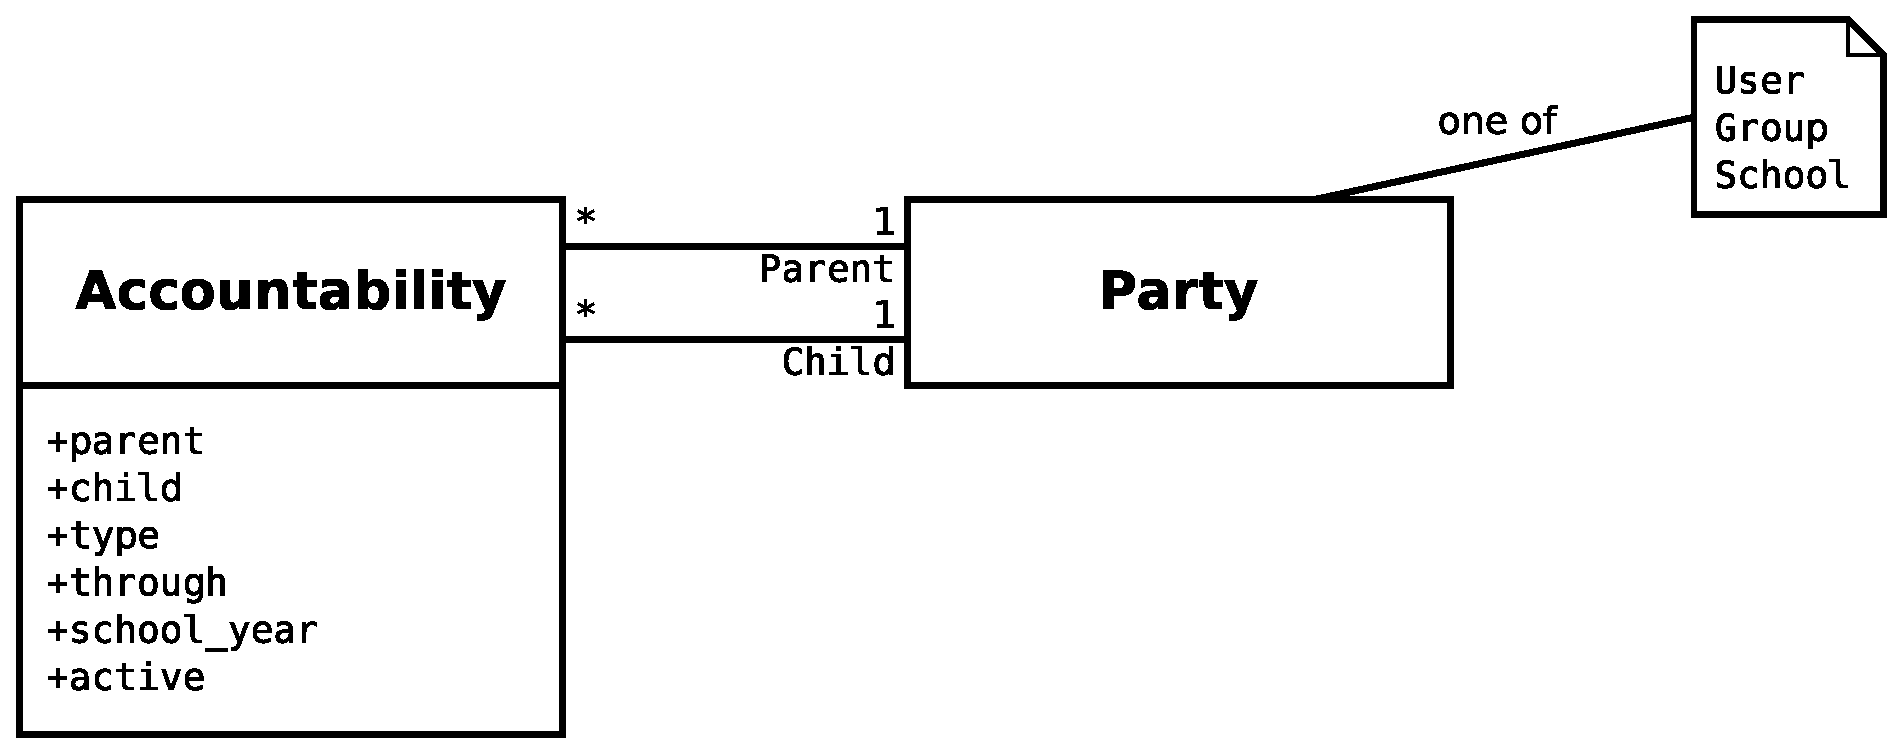
\includegraphics[width=115mm]{social_network_conceptual}
  \caption{Accountability Implementation for User Network.}
  \label{fig:social_network_conceptual}
\end{figure}

For performance reasons (explained in \ref{sec:fa_social_network_impact_analysis}), a series of different AccountabilityTypes were created, in order to cater to a multitude of relationship types, as described in Table~\ref{table:accountability_types}

%\begin{itemize}
%  \item \textbf{group\_professor:} establishes a connection between a \emph{Group} and a \emph{Professor}, meaning that the user is one of the teacher of \emph{Group}
%  \item \textbf{professor:} establishes a connection between two \emph{Users} --- a \emph{Professor} and a \emph{Student} --- creating a teacher-student relationship between them through whichever \emph{Group} they are related to
%  \item \textbf{group\_student:} establishes a connection between a \emph{Group} and a \emph{Student}, meaning that the user is part of the \emph{Group} and taught by the \textbf{group\_professors} associated with the aforementioned \emph{Group}
%  \item \textbf{school\_professor:} establishes a connection between a \emph{School} and a \emph{Professor}
%  \item \textbf{school\_student:} establishes a connection between a \emph{School} and a \emph{Student}
%  \item \textbf{parent:} establishes a parenthood relationship between two users
%  \item \textbf{school\_coordinator:} dictates an \emph{User} is a coordinator (also known as an administrator) of a certain \emph{School}
%  \item \textbf{colleague:} establishes a connection between two \emph{Users} --- either a \emph{Coordinator} or a \emph{Professor} --- through a \emph{School} they both work in
%  \item \textbf{student:} establishes a relationship between a \emph{Coordinator} and a \emph{Student} through a \emph{School}
%  \item \textbf{school\_parent:} establishes a relationship between a \emph{Coordinator} and a \emph{Parent} through a \emph{School}
%  \item \textbf{friend:} establishes a connection between any two \emph{Users} of the system --- whichever their roles may be --- to indicate a friendship relation exists between them
%\end{itemize}

% generated with http://truben.no/latex/table/

\begin{center}
  \begin{small}
    \begin{longtable}{|l|l|l|l|p{5cm}|}
      \hline
      \textbf{Type}      & \textbf{Parent} & \textbf{Child} & \textbf{Through} & \textbf{Description} \\
      \hline \hline
      group\_professor   & Group           & Professor      & ---              & establishes a connection between a \emph{Group} and a \emph{Professor}, meaning that the user is one of the teachers of \emph{Group} \\ \hline
      professor          & Professor       & Student        & Group            & establishes a connection between two \emph{Users} --- a \emph{Professor} and a \emph{Student} --- creating a teacher-student relationship between them through whichever \emph{Group} they are related to \\ \hline 
      group\_student     & Group           & Student        & ---              & establishes a connection between a \emph{Group} and a \emph{Student}, meaning that the user is part of the \emph{Group} and taught by the \textbf{group\_professors} associated with the aforementioned \emph{Group} \\ \hline 
      school\_professor  & School          & Professor      & ---              & establishes a connection between a \emph{School} and a \emph{Professor} \\ \hline 
      school\_student    & School          & Student        & ---              & establishes a connection between a \emph{School} and a \emph{Student} \\ \hline 
      parent             & Parent          & Student        & ---              & establishes a parenthood relationship between two users \\ \hline 
      school\_cordinator & School          & Coordinator    & ---              & dictates an \emph{User} is a coordinator (also known as an administrator) of a certain \emph{School} \\ \hline 
      colleague          & Professor       & Coordinator    & School           & establishes a connection between two \emph{Users} --- either a \emph{Coordinator} or a \emph{Professor} --- through a \emph{School} they both work in \\ \hline 
      student            & Coordinator     & Student        & School           & establishes a relationship between a \emph{Coordinator} and a \emph{Student} through a \emph{School} \\ \hline 
      school\_parent     & Coordinator     & Parent         & School           & establishes a relationship between a \emph{Coordinator} and a \emph{Parent} through a \emph{School} \\ \hline 
      friend             & User            & User           & ---              & establishes a connection between any two \emph{Users} of the system --- whichever their roles may be --- to indicate a friendship relation exists between them \\ \hline
    
    \caption{AccountabilityTypes created to describe every type of existent relation.}
    \label{table:accountability_types}
    \end{longtable}
  \end{small}
\end{center}

Some of the aforementioned AccountabilityTypes are representative of every type of interpersonal relationship existent in the escolinhas.pt platform. At first sight, some of the AccountabilityTypes created may seem redundant, such as student and school\_parent: they exist because the school coordinator needs to be able to contact everyone who is part of the school. One could argue these connections could easily be inferred through the relations between the coordinator and his or her school, and the relations existent between the school and its students, and finally use the existent parenthood relationships. However, as described in \ref{sec:fa_social_network_variability_requirements}, one of the major design flaws (regarding variability), was the completely dynamic nature of the contacts network --- as the network was always built upon request, there was no viable way of modifying it without using hardcoded rules or a configuration setup external to the code. Thus, the choice to implement apparently redundant AccountabilityTypes tied itself with the necessity to have full control over the existent social relationships. The remainder of the AccountabilityTypes are used to store and facilitate access to membership-like relationships, by stating a certain user is part of a school or group at a given school year. This also allows the platform to keep a history of past (inactive) relationships between entities in the system.

\subsection{Impact Analysis}\label{sec:fa_social_network_impact_analysis}

The usage of this design pattern not only solved some of the existing variability and performance problems, but introduced a new possibility: the ability to create relationships between any two entities in the system. This leads to a very flexible network, capable of being modified at the M0 (data) level (see \ref{sec:aom_architecture}), which is a pre-requisite for end-user level variability.

A second objective pertaining to the application of this pattern was to improve the performance related to contact list creation and the identification of these before the user. This task is currently extremely expensive, with an edge case of 5724 queries needed to fetch and identify 715 contacts. A user with only 18 contacts generates 154 queries. This means that an average of 8 queries are performed for each one of the contacts, meaning the cost of this operation is approximately linear in nature, as depicted in Fig.~\ref{fig:contact_queries}.

\begin{figure}[H]
  \centering
  \includegraphics[width=125mm]{graphs/contact_queries}
  \caption{Average number of queries performed per number of contacts.}
  \label{fig:contact_queries}
\end{figure}

The graph in Fig.~\ref{fig:contact_queries} represents the average number of queries performed per number of contacts a user has, and it was sampled from a random population of 10000 real users of the platform. As stated before cost growth of the function is only approximately linear: due to the dynamic nature of the network, some users may have a sparser network --- e.g. less groups associated with, but more users associated with each group the user is part of --- which can explain the unexpected decrease in the number of queries around the 200-mark and the irregularities in users with less than 100 contacts. However, in practice, this cost can be extrapolated to a linear cost, to a point where one can infer that the number of queries performed is approximately 8 times the number of contacts, which represents a very serious performance issue for one of the most used features of the platform.

%The data used to build the chart can be found in \nameref{sec:appendix_a}

The implementation of the \textsc{Accountability} pattern to maintain the relationships between users was able to reduce the cost of the abovementioned task to from $O(n)$ (Fig.~\ref{fig:contact_queries}) $O(1)$: by using the RoR \textsc{ActiveRecord} API to access and manipulate these connections, only 11 queries are performed to fetch and identify an user contacts, regardless of the size of said contact list. This means that the platform is able to sustain a considerable growth without suffering serious impacts on the performance of seemingly trivial operations.


\section{Documents}\label{sec:fa_documents}

\subsection{Variability Requirements}\label{sec:fa_documents_variability_requirements}

The document editor present in \emph{escolinhas.pt} is one of the core components of the system and one of the used features of the platform. This being the case, and due to the constantly evolving nature (\textbf{FIXME: it's not the nature that constantly evolves, but the product}), it is also one of the most modified parts of the system. As it can be seen in Fig.~\ref{fig:documents_current}, this structure has to grow both in size and complexity every time a new type of block content is introduced --- represented by the gray entities in Fig.~\ref{fig:documents_current}. This means that whenever a new type of content is introduced in the system, which happens somewhat frequently --- from three types of blocks (\emph{Paragraphs}, \emph{Drawings} and \emph{ImageDocuments/Photos}) in September 2009 to seven in April/May 2010 --- it is necessary to setup a new \textsc{ActiveRecord} class (along with all the logic for versioning) and a new \textsc{Controller} to accept the requests necessary to create, edit or delete any of these entities. Despite working as intented, this workflow is not adequate to the constant evolution and prototyping the document editor is subjected to.

\begin{figure}[H]
  \centering
  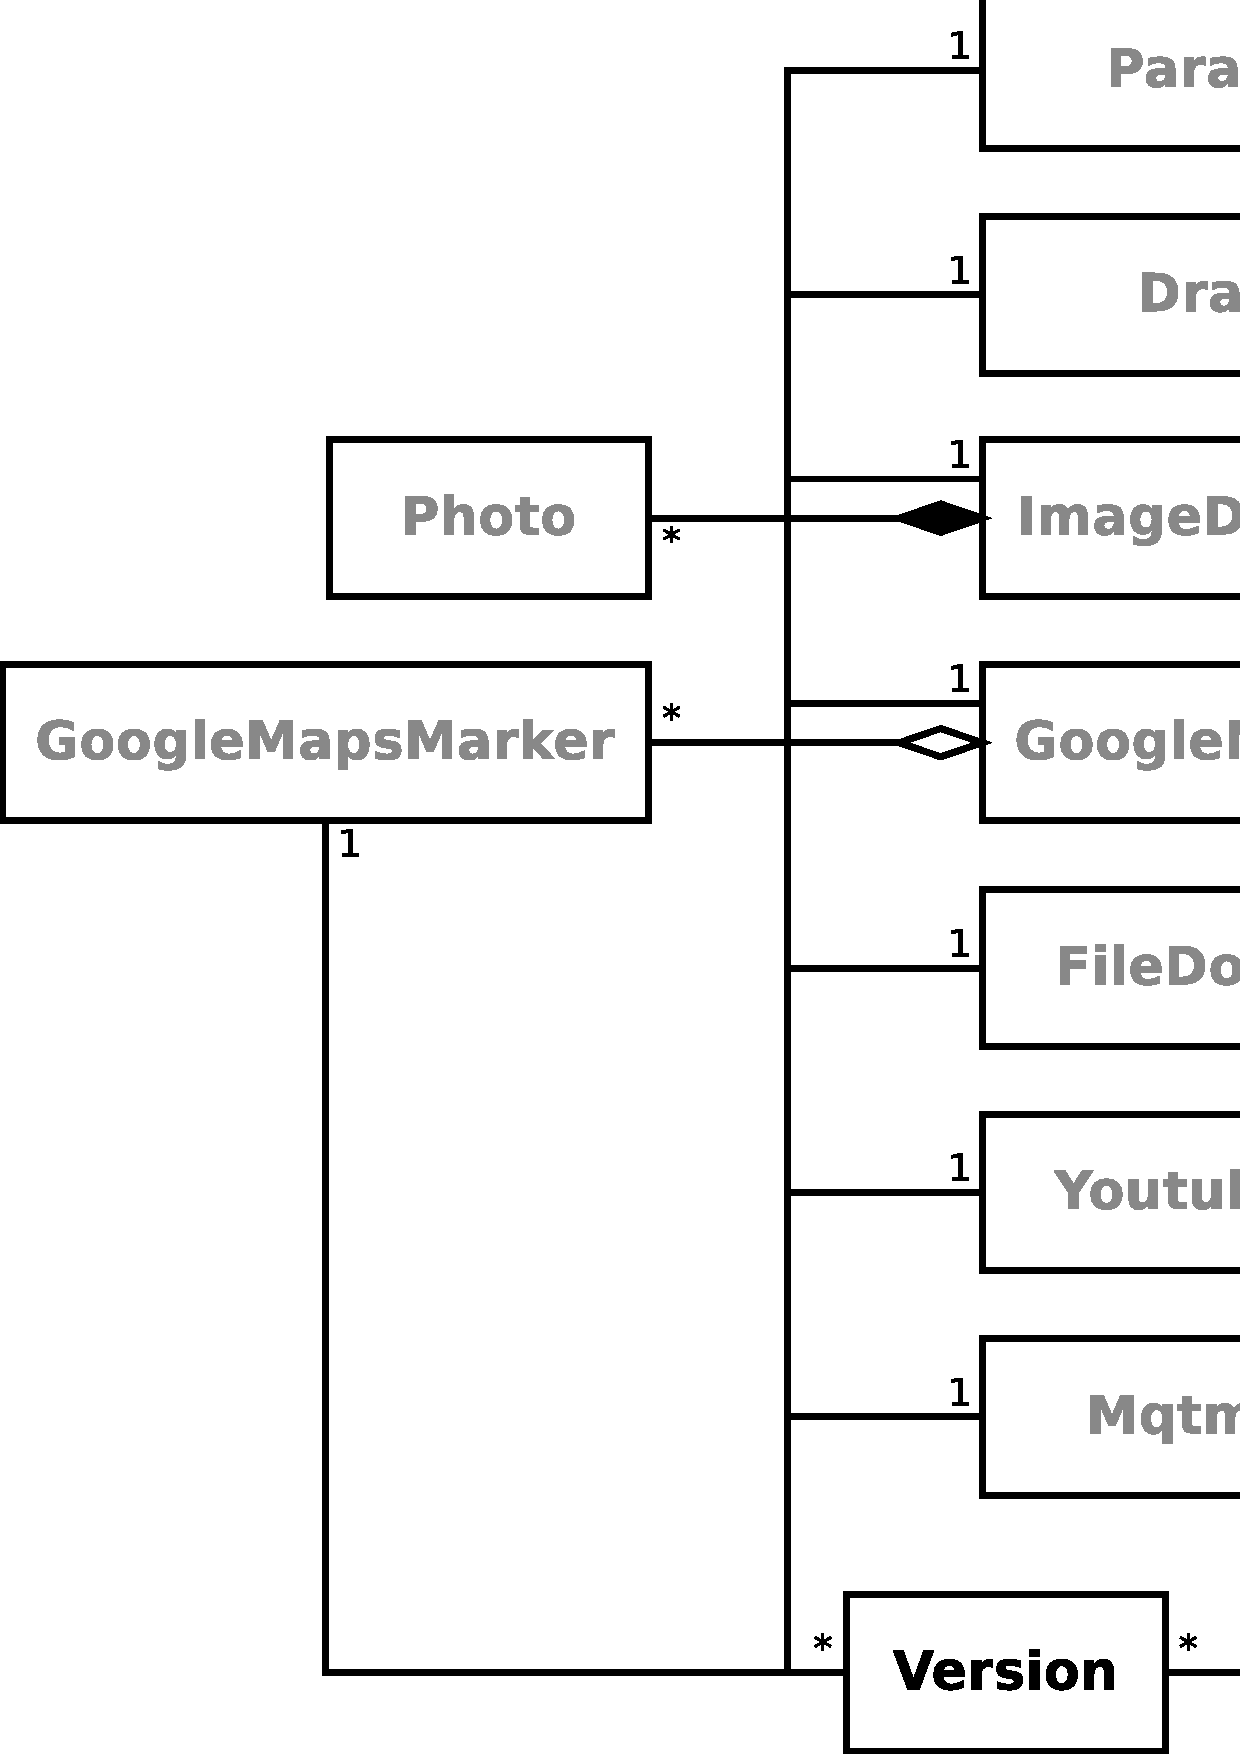
\includegraphics[width=165mm]{documents_current.pdf}
  \caption{Current Documents Model}
  \label{fig:documents_current}
\end{figure}

\subsection{Candidate Patterns}\label{sec:fa_documents_candidate_patterns}

\subsection{Chosen Patterns \& Rationale}\label{sec:fa_documents_chosen_patterns_rationale}

The pattern used is a composite design pattern \cite{riehle_composite_patterns}, where various smaller design patterns work in tandem to create a more complex pattern.

\begin{figure}[H]
  \centering
  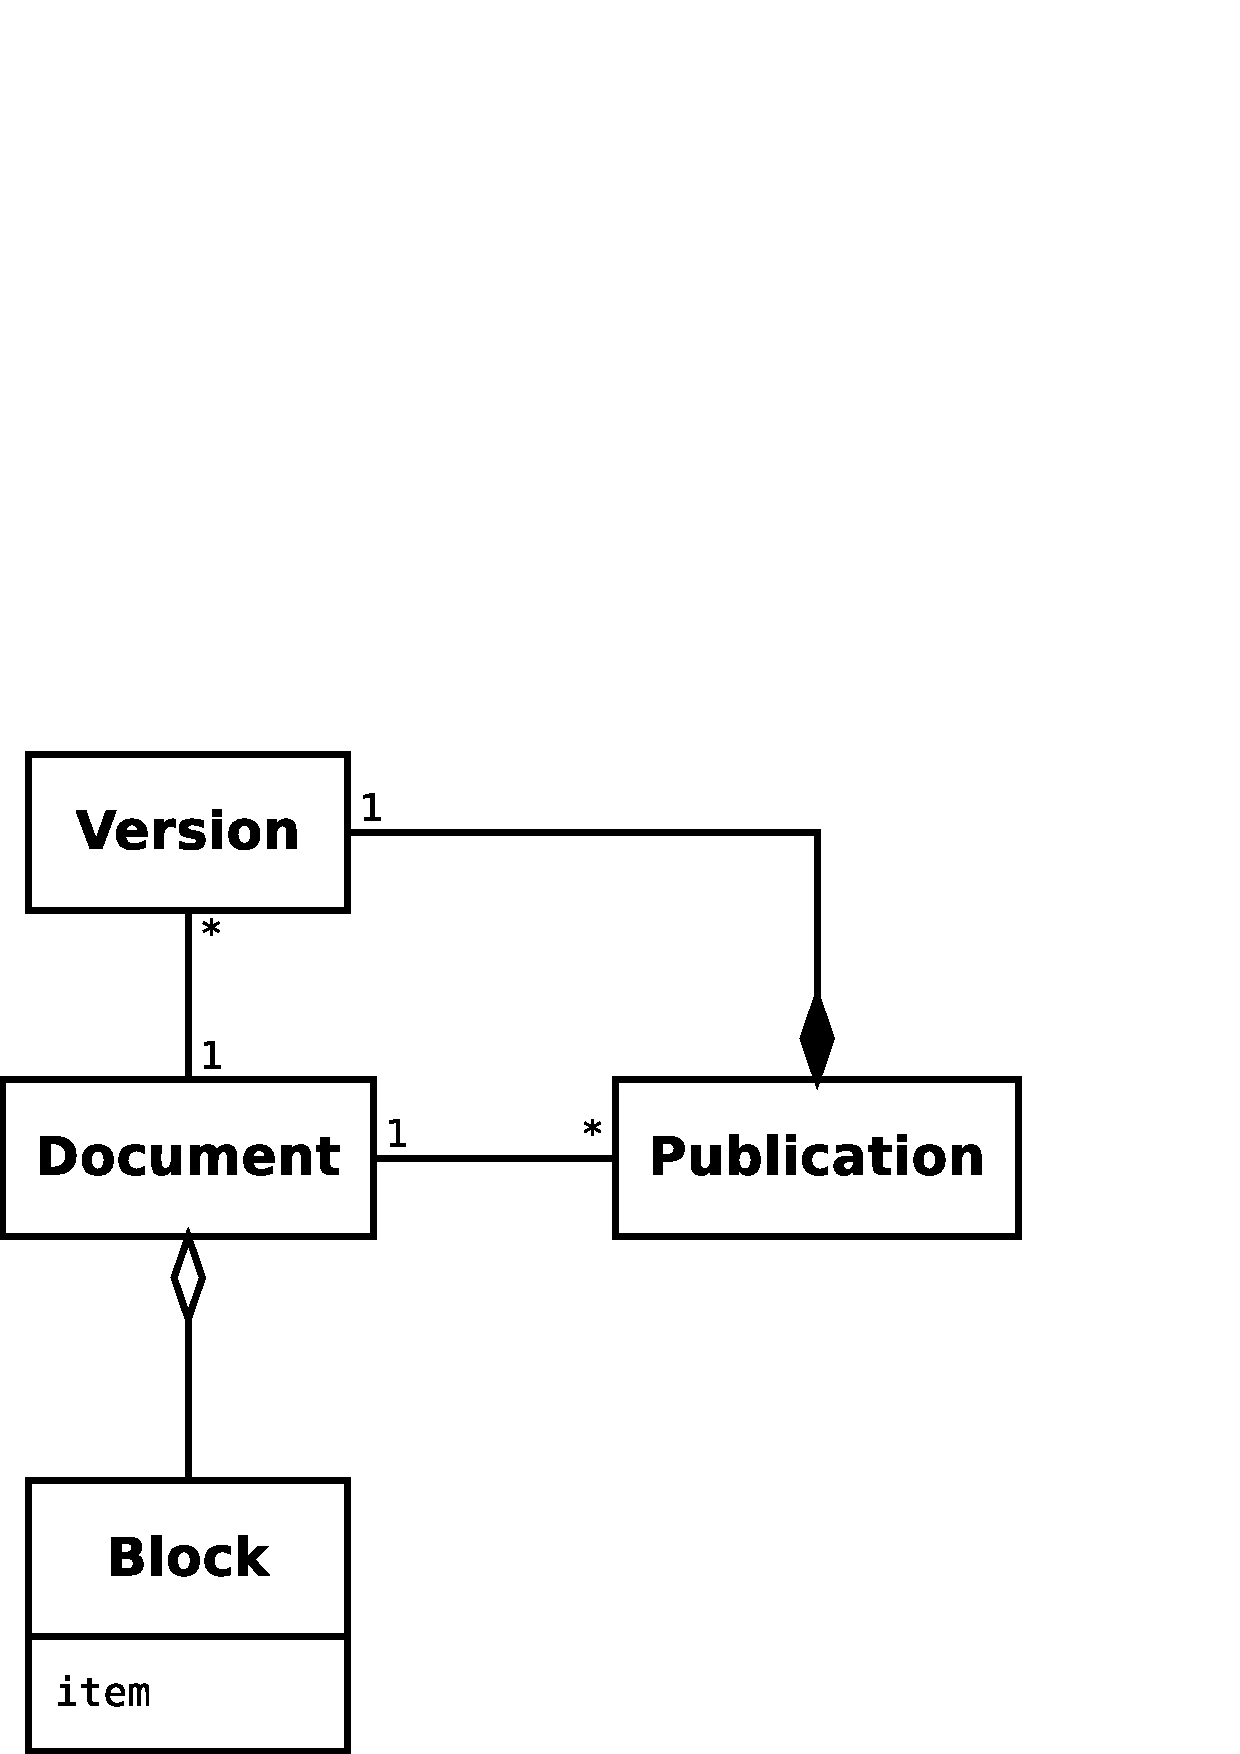
\includegraphics[width=75mm]{documents_conceptual.pdf}
  \caption{Conceptual Documents Model}
  \label{fig:documents_conceptual}
\end{figure}

\textbf{FIXME}

patterns used
\begin{itemize}
  \item \textsc{Memento} - used for versioning
  \item \textsc{Property} (simplified variant) - used for decoupling the type of the block item from the database schema
  \item \textbf{INVESTIGATE: pattern 3} - the fact that a \emph{Publication} points to a specific \emph{Version} of a \emph{Document} may be a pattern --- it works as a \emph{tag} in a VCS (version control system) system such as git or SVN.
\end{itemize}

The variant of the \textsc{Property} pattern implemented is simplified to the highly dynamic nature of the Ruby language --- which means that, for this particular problem, it is able to build new types of objects or even create new class definitions in runtime.

\subsection{Implementation}\label{sec:fa_documents_implementation}

\subsection{Impact Analysis}\label{sec:fa_documents_impact_analysis}


\chapter{Conclusions}\label{chap:conclusions}

The research developed for this initial stage provides a solid knowledge base, providing an overview of existing methods and technologies.

The technologies chosen should not prove an obstacle to the development, as most of them are open-source, with good, helpful documentation and have a strong, active community.

Finally, it is possible to conclude the objectives relative to the problem study, state of the art and technology analysis are fully completed, as well as the planning relative to the project development and dissertation writing.



%%----------------------------------------
%% Final materials
%%----------------------------------------

\begin{singlespace}
  %% Bibliography
  %% Comment the next command if BibTeX file not used,
  %% bibliography is in ``myrefs.bib''
  \PrintBib{thesis}

  %% Index
  %% Uncomment next command if index is required,
  %% don't forget to run ``makeindex mieic'' command
  %\PrintIndex

  %% Comment next 2 commands if numbered appendixes not used
  \appendix
  \chapter{Unique Users Since September 1st, 2010}\label{appendix:unique_visitors}

\begin{figure}[H]
  \includegraphics[width=150mm]{escolinhas_unique_visitors}
  \caption{Number of unique visitors per month, since September 1st, 2010, extracted from Google Analytics.}
  \label{fig:unique_visitors}
\end{figure}

\begin{table}
  \begin{center}
    \begin{tabular}{|l|l|}
      \hline
      \textbf{Date}     & \textbf{Visitors} \\
      \hline
      September 1, 2010 & 720  \\ \hline
      October 1, 2010   & 1241 \\ \hline
      November 1, 2010  & 1819 \\ \hline
      December 1, 2010  & 1672 \\ \hline
      January 16, 2011  & 1006 \\
      \hline
    \end{tabular}
    \caption{Number of unique logged in visitors per month, since September 1st, 2010.}
    \label{table:unique_visitors}
  \end{center}
\end{table}

\vspace{10cm}


\end{singlespace}

\end{document}

